\chapter{Projektafgrænsning (JS)}

Grundet begrænset tid og ressourcer er det nødvendig fra start at sætte nogle begrænsninger til hvilke dele af systemet der ønskes realiseres, som det ligeledes har været nødvendigt under forløbet at skære ned på hvad vi har ønsket realiseret. 

X10 opererer normalt på 230 V nettet, men da vi ikke har autoritet til at arbejde med 230 V og af sikkerhedsmæssige årsager foregår realiseringen ved 18 V 50 Hz. Dette ændrer ikke på funktionaliteten eller virkemåden af systemet. 

Lyddetektionen er desværre ikke nået realiseret som ønsket. Det er i stedet lavet med en knap der giver et højt signal som skal imitere at lyd er detekteret. Se figur \ref{fig:BABY_ALARM}. 

\begin{figure}[htbp]
  \centering
    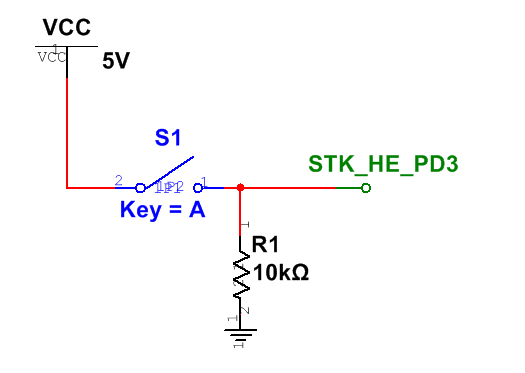
\includegraphics[width=0.5\textwidth]{billeder/BABY_SWITCH}
    \caption{Schematic over knap for lyddetektion}
    \label{fig:BABY_ALARM}
\end{figure}

